\documentclass[../../spr.tex]{subfiles}

\begin{document}


\section{Implementacja}

\subsection{Opis głównych funkcjonalności aplikacji}

Aplikacja do zarządzania siłownią została zaprojektowana z myślą o różnych rolach użytkowników: klientach, pracownikach, trenerach oraz menadżerach. W zależności od przypisanej roli dostępne są różne funkcjonalności.

\begin{itemize}
  \item \textbf{Klient} może:
  \begin{itemize}
    \item Przeglądać status swojego karnetu.
    \item Śledzić swój postęp treningowy.
    \item Przeglądać i zapisywać się na dostępne sesje treningowe.
    \item Przeglądać historię treningów.
  \end{itemize}

  \item \textbf{Menadżer} ma możliwość:
  \begin{itemize}
    \item Tworzenia nowych pracowników poprzez formularz.
    \item Przeglądania listy klientów i pracowników.
    \item Zarządzania salami treningowymi oraz zadaniami serwisowymi.
  \end{itemize}
    \item \textbf{Pracownik} ma możliwość:
  \begin{itemize}
    \item Przeglądania listy klientów.
    \item Sprawdzania ważności karnetów.
    \item Zgłaszania usterek i tworzenia zadań serwisowych.
  \end{itemize}

  \item \textbf{Trener} może:
  \begin{itemize}
    \item Przeglądać przypisanych podopiecznych.
    \item Tworzyć i edytować plany treningowe.
    \item Zarządzać kalendarzem sesji treningowych.
  \end{itemize}

\end{itemize}

Aplikacja obsługuje różne widoki dla użytkowników w zależności od ich roli i zapewnia prosty oraz intuicyjny interfejs użytkownika, co przedstawiono na poniższych zrzutach ekranu.

\subsection{Prezentacja zrzutów ekranu (screeny) prezentujących działanie aplikacji}

\begin{figure}[H]
  \centering
  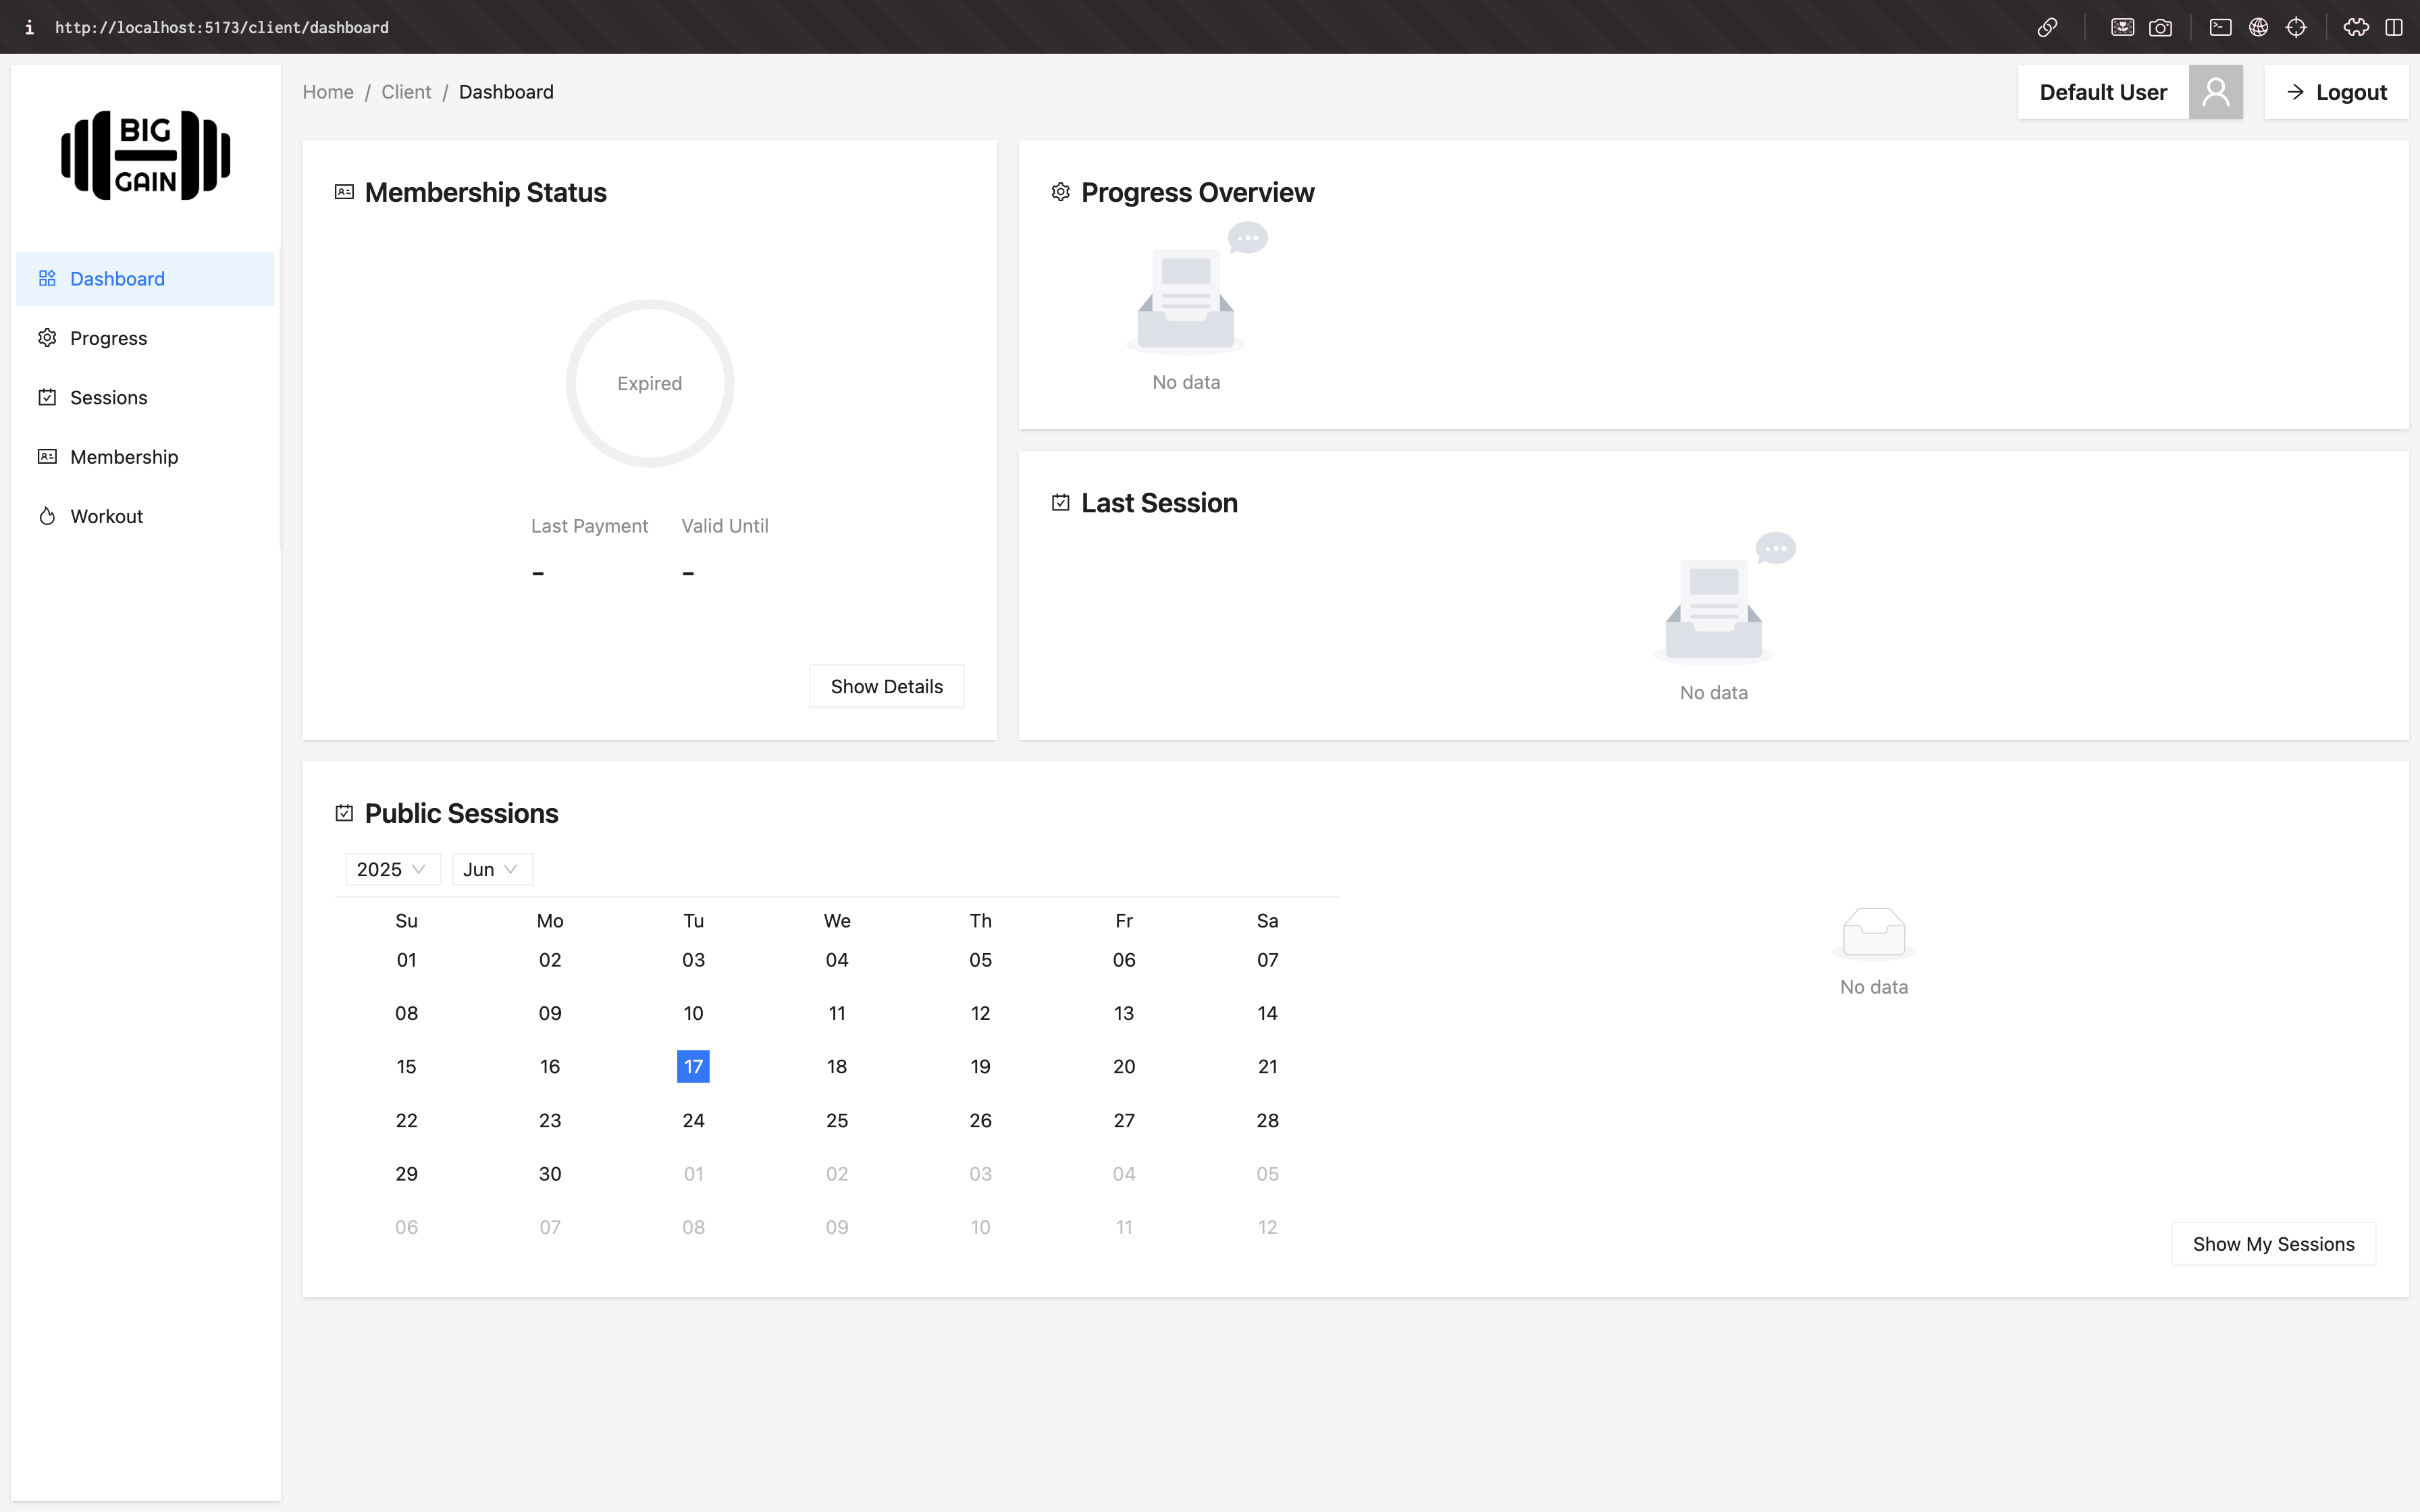
\includegraphics[width=0.95\textwidth]{client.png}
  \caption{Panel klienta – przegląd statusu członkostwa, progresu oraz kalendarz sesji.}
\end{figure}

\begin{figure}[H]
  \centering
  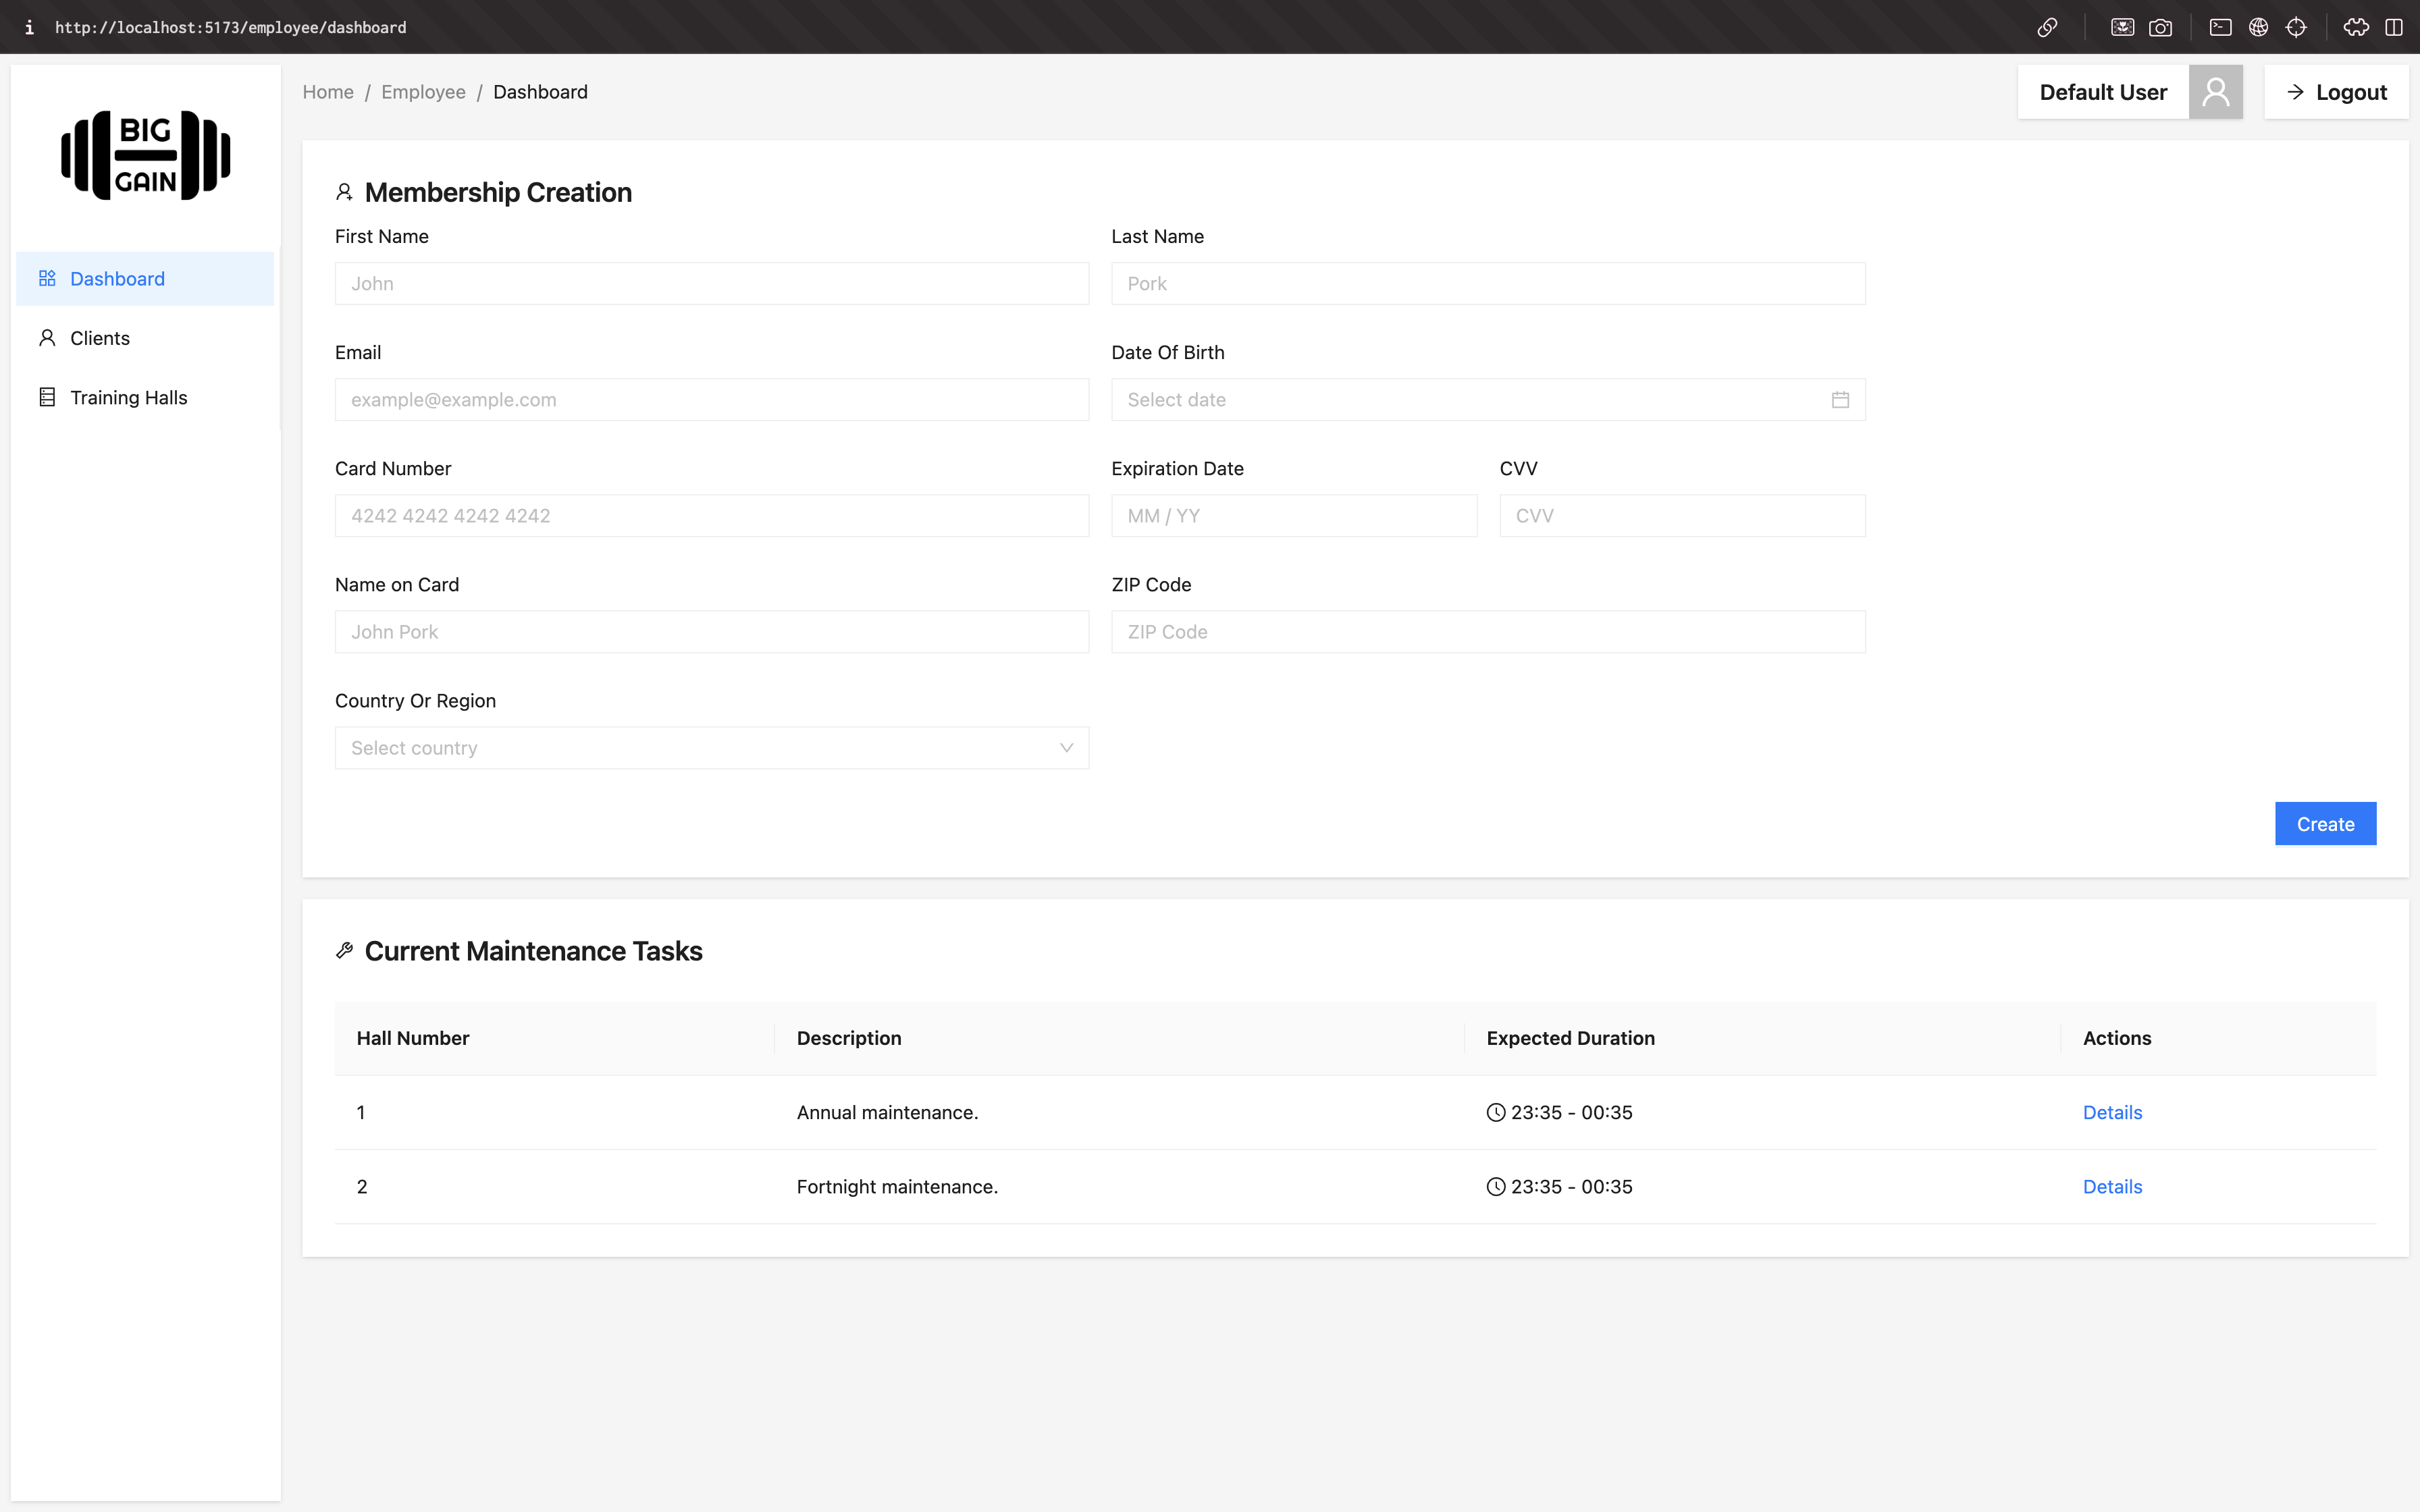
\includegraphics[width=0.95\textwidth]{pracownik.png}
  \caption{Panel pracownika – .}
\end{figure}

\begin{figure}[H]
  \centering
  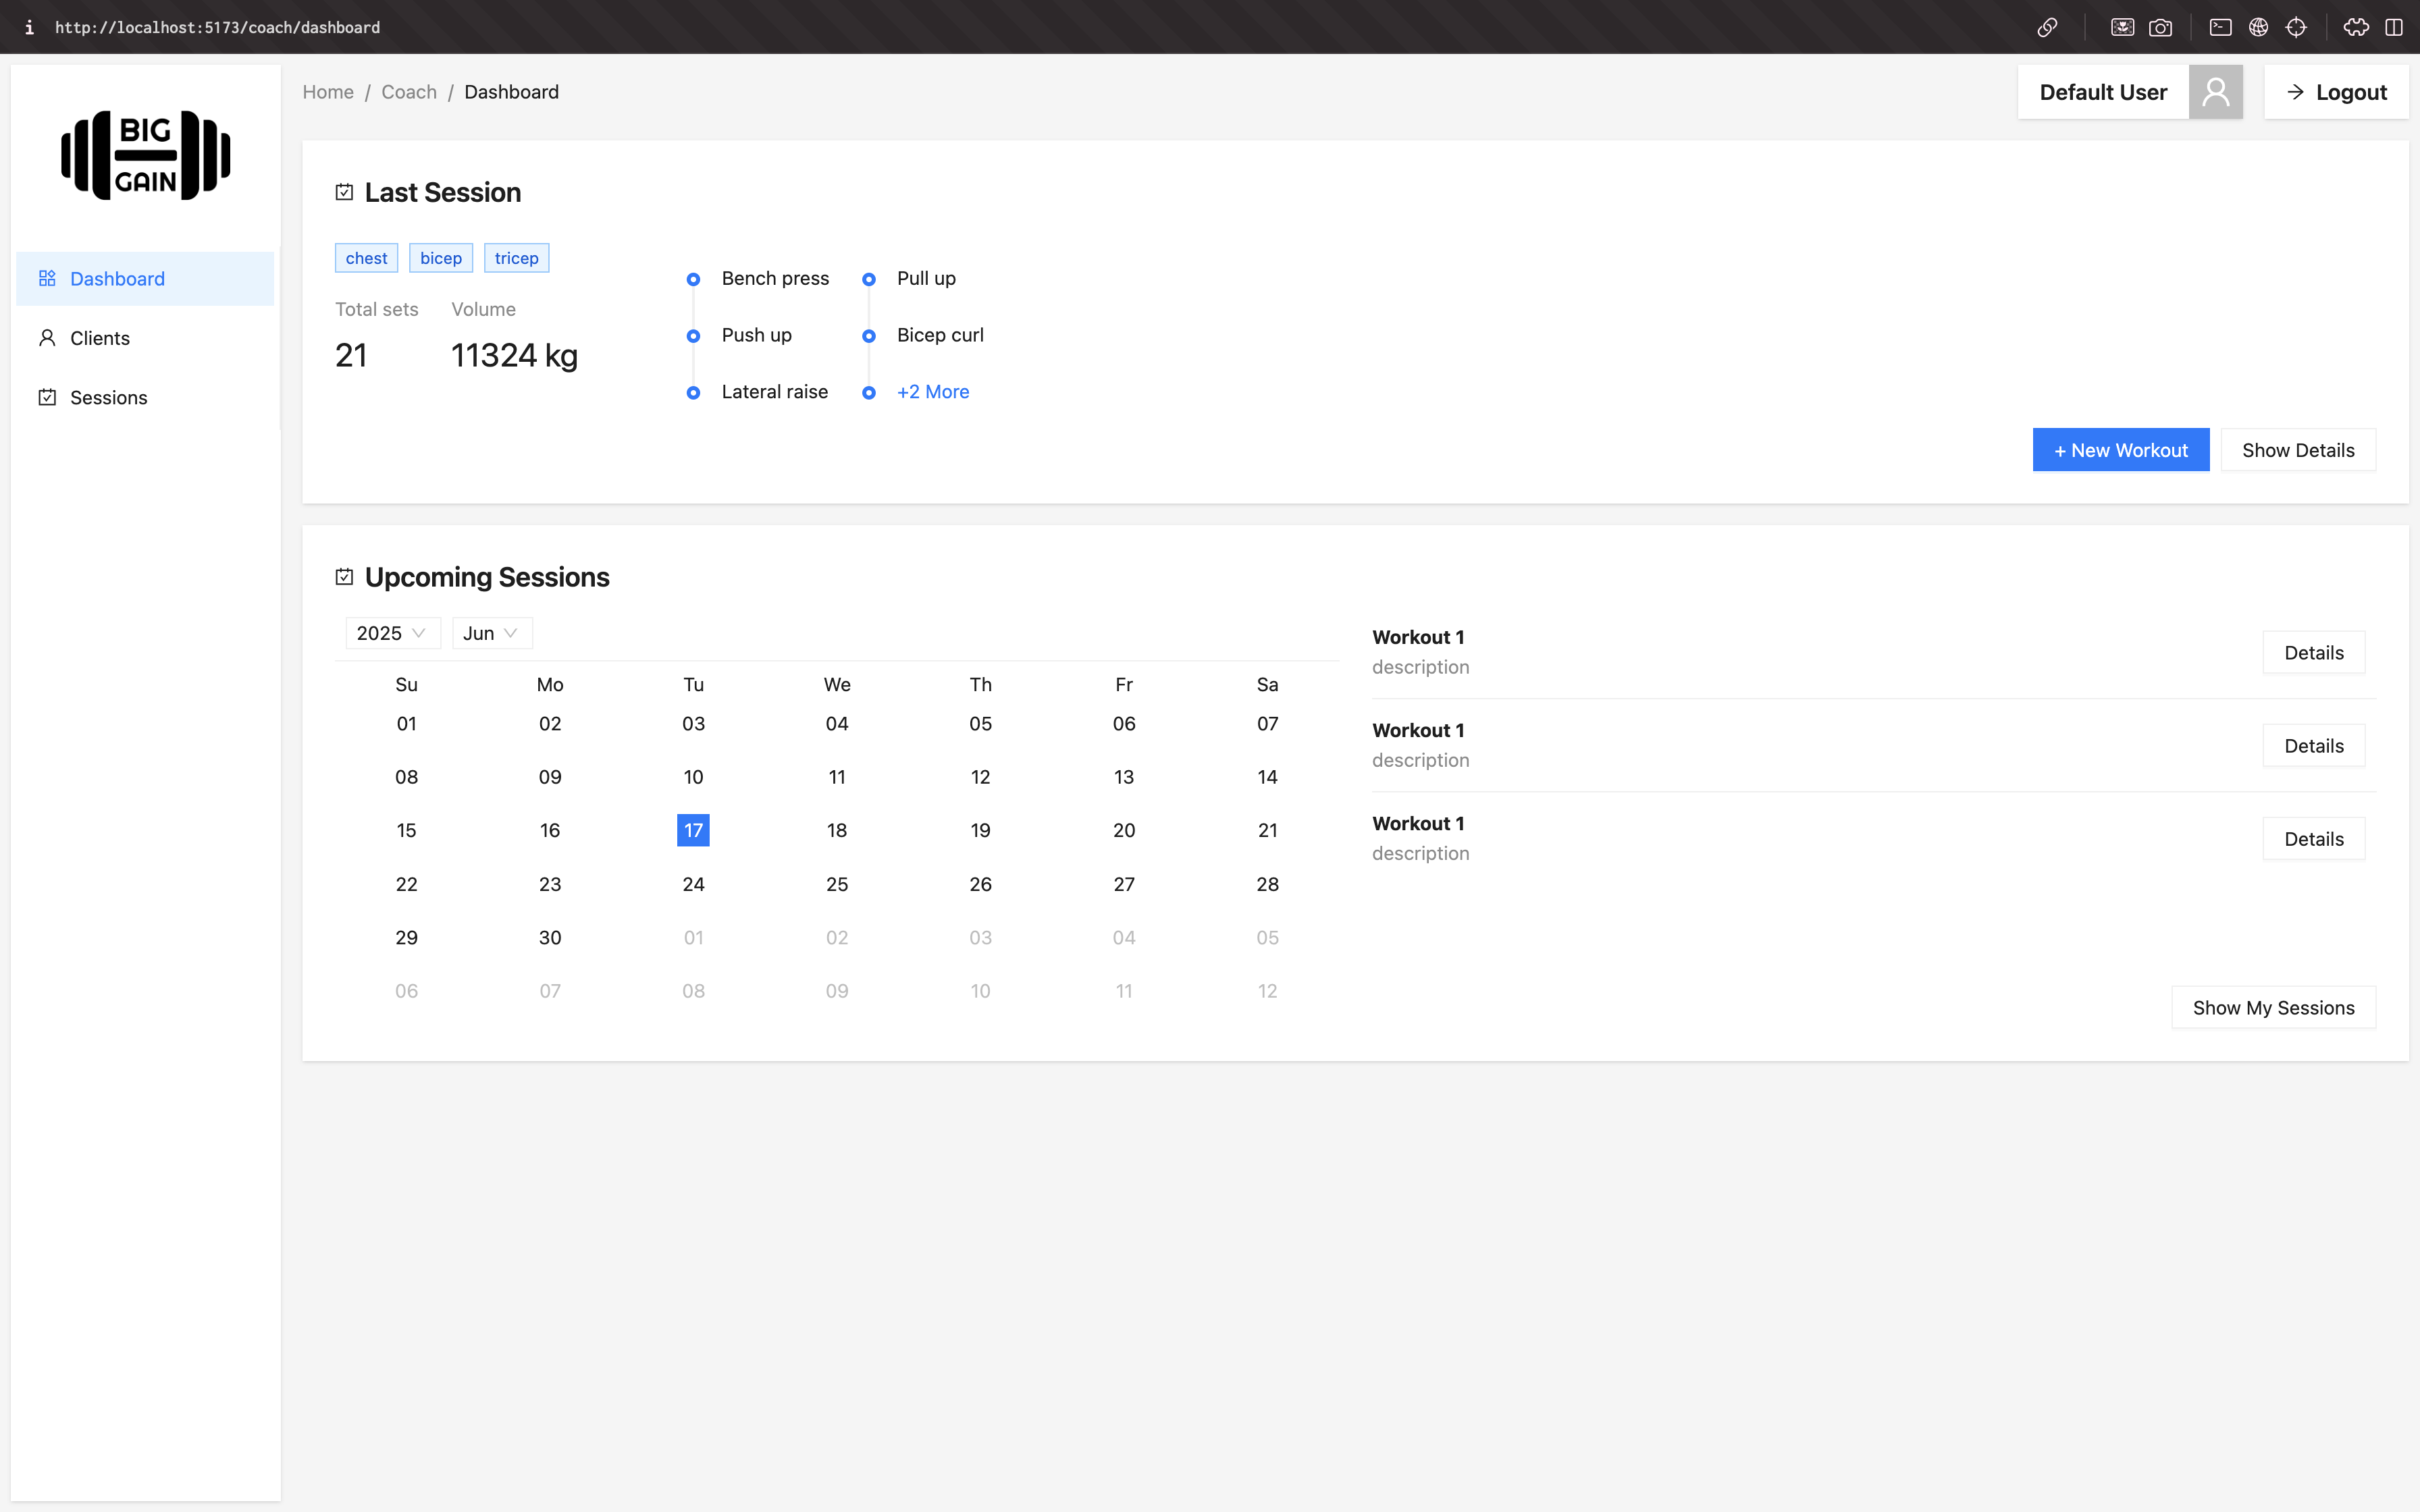
\includegraphics[width=0.95\textwidth]{trener.png}
  \caption{Panel trenera – .}
\end{figure}

\begin{figure}[H]
  \centering
  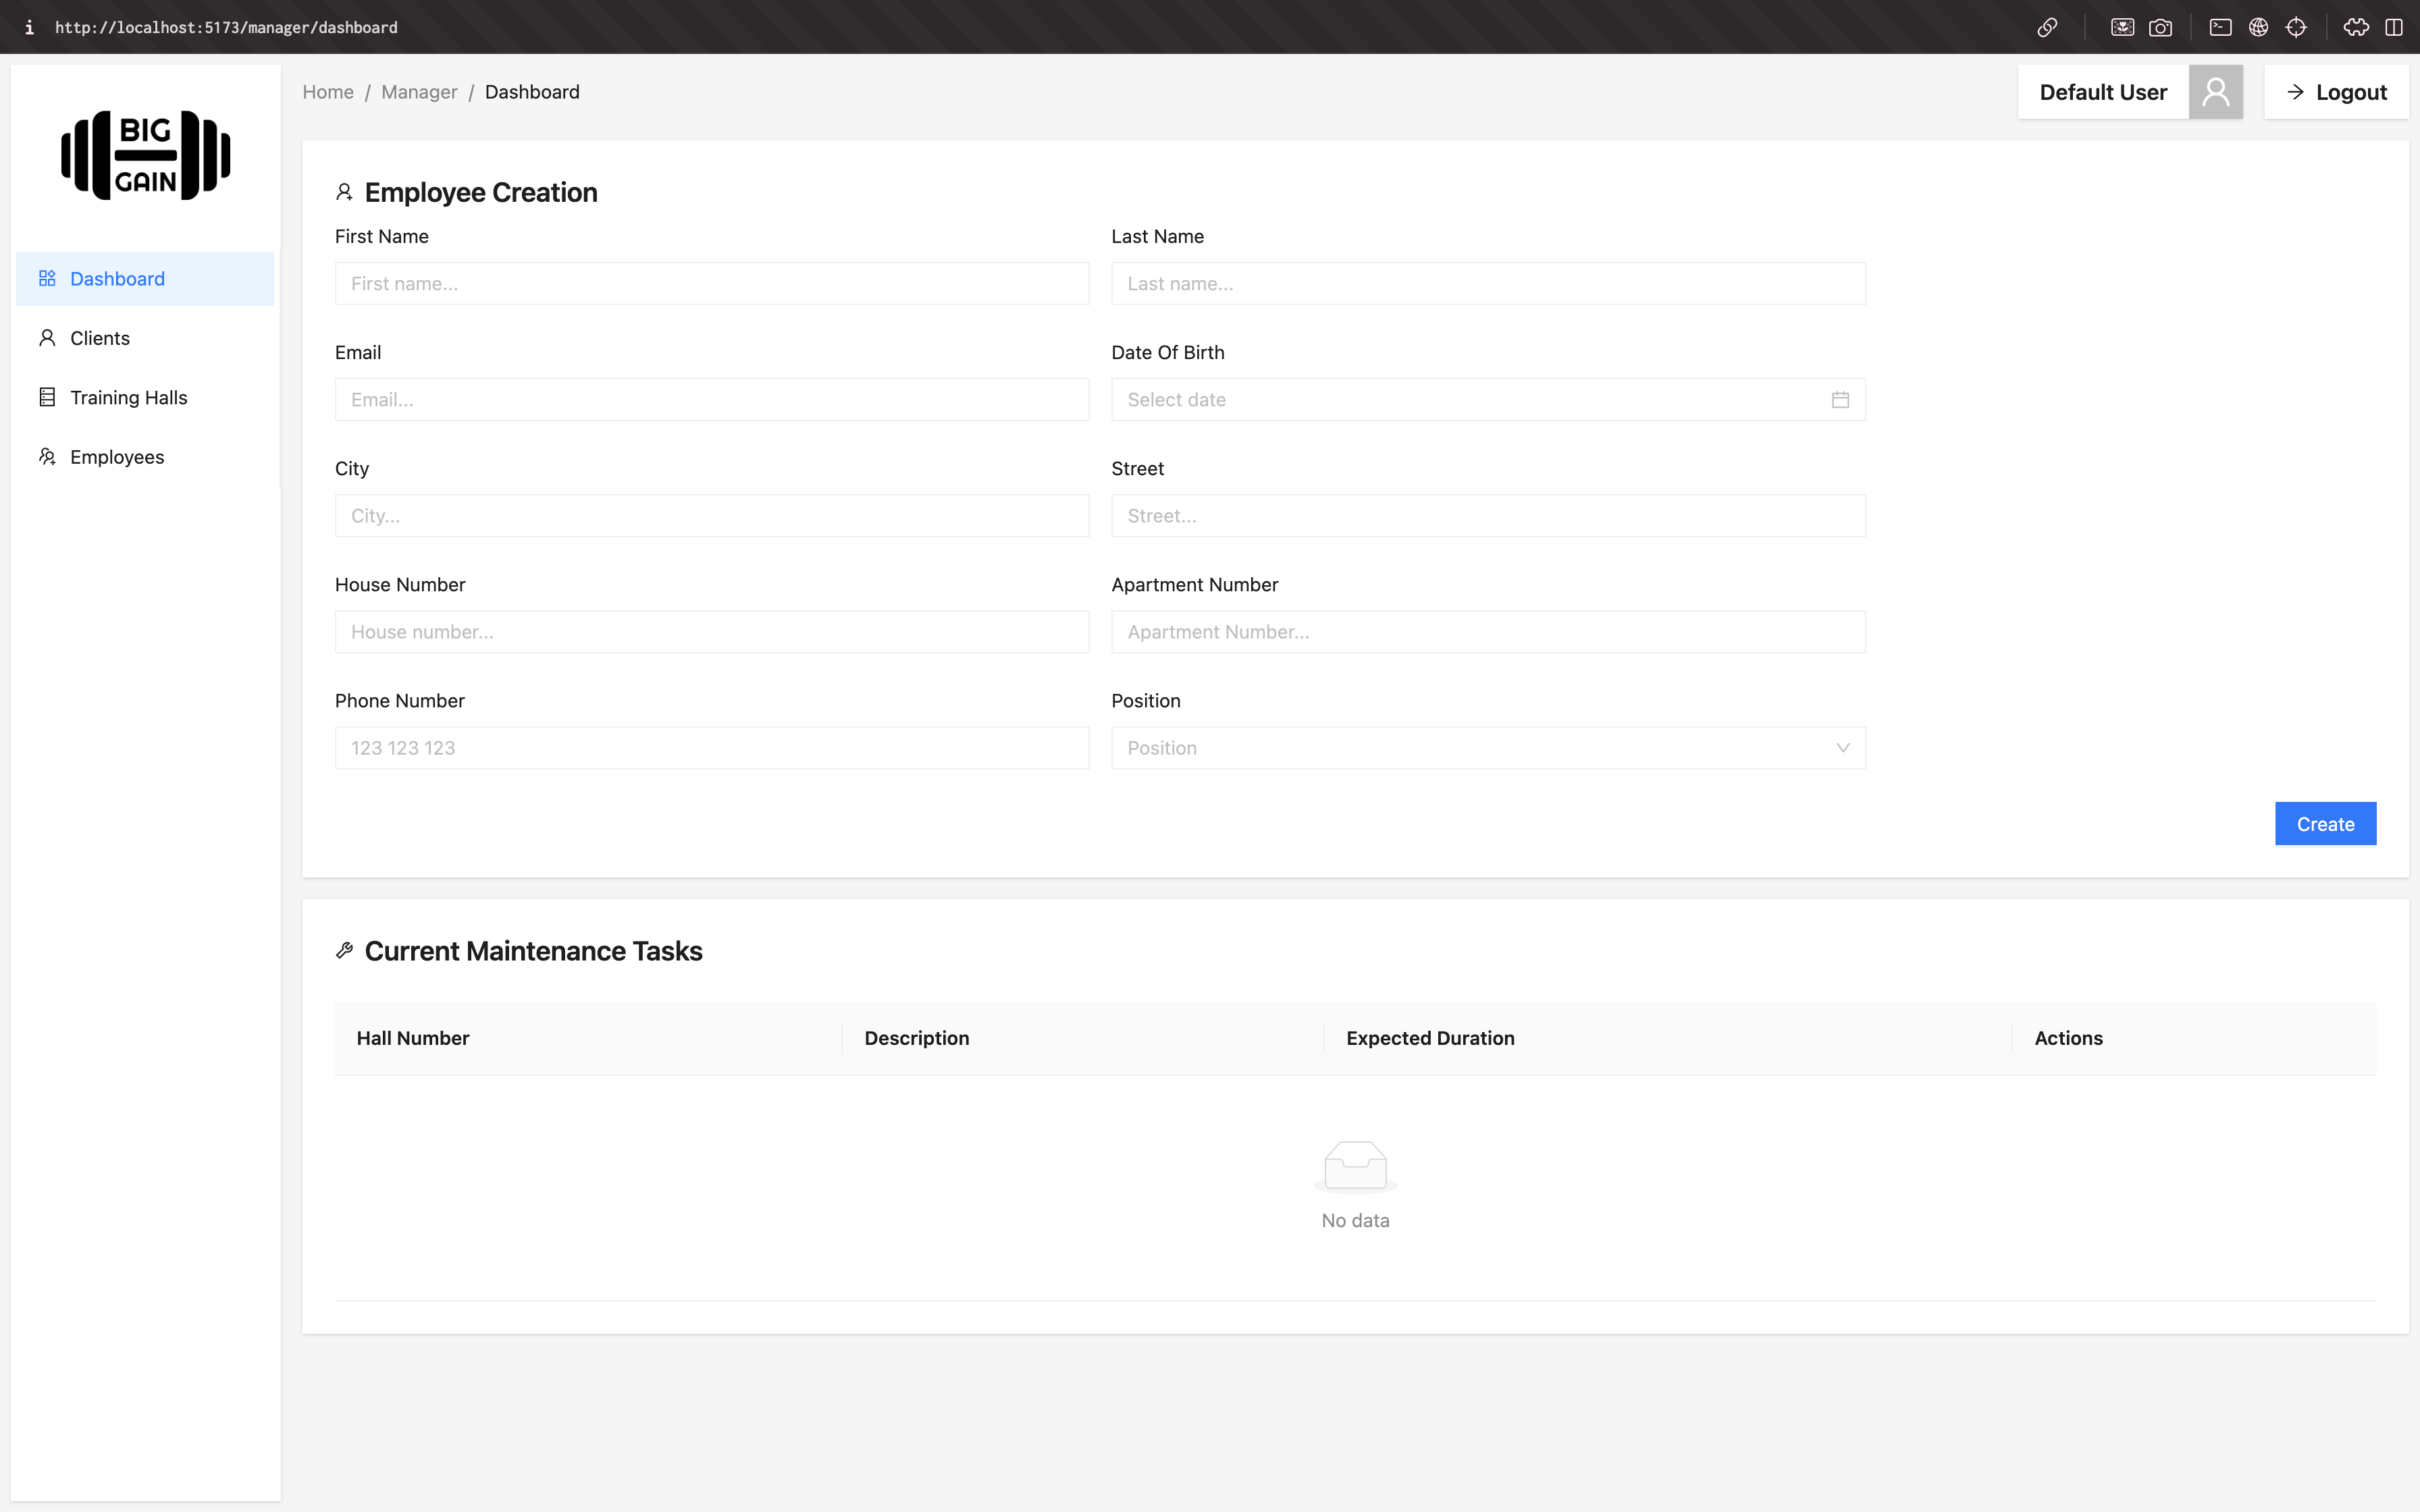
\includegraphics[width=0.95\textwidth]{menadzer.png}
  \caption{Panel menadżera – tworzenie nowego pracownika oraz przegląd aktualnych zadań serwisowych.}
\end{figure}

\subsection{Wybrane fragmenty kodu z kluczowymi funkcjonalnościami}

Poniższy komponent React odpowiada za formularz tworzenia nowej sali treningowej.
Został on zaimplementowany z użyciem biblioteki \texttt{Ant Design} i
umożliwia menadżerowi dodanie nowej sali do systemu poprzez wprowadzenie jej numeru,
wybranie typu oraz podanie opisu.

\inputminted[breaklines, fontsize=\footnotesize, breakanywhere]
{typescript}{./sections/implementacja/HallCreationCard.tsx}




\end{document}